\chapter{IMPLEMENTASI DAN PENGUJIAN}
\section{Lingkungan Implementasi}
\par
Sesudah menyelesaikan proses analisis, proses yang dilakukan selanjutnya adalah perancangan spesifikasi. Perancangan spesifikasi ini dilakukan untuk merancang kebutuhan-kebutuhan perankat keras dan perangkat lunak pada aplikasi yang dibangun.
\subsection{Perangkat Keras}
\par
Berikut pada tabel \ref{perangkatker} merupakan spesifikasi yang digunakan pada proses penelitian proyek I.

\begin{table}[!htbp]
\captionsetup{singlelinecheck=off}
\caption{Deskripsi Perangkat Keras}
\label{perangkatker}
\begin{tabular}{|l|l|l|l|}
\hline
No & Nama Perangkat & Spesifikasi & Keterangan \\
\hline

1 &  \textit{Harddisk} & 500 GB  & Media untuk menyimpan \\
 & & & data aplikasi yang dibuat  \\
\hline

2 &  \textit{Memory} & 4 GB & \textit{Memory System} yang digunakan  \\
\hline

3 &  \textit{processor} & \textit{Intel® core™ i5-8250U  } &  Untuk kecepatan transfer data dari \\

 & & \textit{CPU @ 1.60GHz} &  sistem yang sangat bergantung \\
 
 & &\textit{(8 CPUs),~1.8Ghz} & pada kecepatan prosesor komputer \\
\hline

4 &  Infrastruktur Jaringan &    & Bisa dianalogikan sebagai \\     & & &  alur proses dari titik awal proses \\
& & & sampai pada akhir proses  \\

\hline
\end{tabular}
\end{table}

\subsection{Perangkat Lunak}
\par
Berikut pada tabel \ref{lunak} merupakan spesifikasi yang digunakan pada proses penelitian proyek I.

\begin{table}[!htbp]
\captionsetup{singlelinecheck=off}
\caption{Deskripsi perangkat Lunak \textit{Client}}
\label{lunak}
\begin{tabular}{|l|l|l|l|}
\hline
No & \textit{Tools} & Fungsi & Keterangan \\
\hline

1 &  \textit{Windows 10} & Sistem Operasi  & -  \\

\hline

2 &  \textit{Xampp 1.7.3} & \textit{server} Basis Data & - \\
\hline

3 &  \textit{Photoshop CS} & desain antar muka & - \\
\hline

4 &  \textit{PHP,HTML,CSS} & \textit{Bahasa Program} & -  \\    
\hline

5 & \textit{sublime text} & software pendukung & - \\
\hline

6 & \textit{google chrome} & \textit{browser} & - \\
\hline
\end{tabular}
\end{table}


\section{Pembahasan Hasil Implementasi}
\par
Berdasarkan pada gambar \ref{flowmapsistem}, dapat dipahami bahwa proses registrasi pada aplikasi CGV-blitz masih memiliki ruang untuk dikembangkan, diantaranya melakukan registrasi menggunakan akun Google+, registrasi akan jauh lebih efektif dan efisien.
\par
Berdasarkan pada gambar 3.19 , fungsi-fungsi bahasa SQL yang digunakan adalah  \textbf{INSERT}, dan \textbf{UPDATE} . Dan bahasa pemrograman \textit{PHP} yang digunakan untuk menghubungkan \textit{website} dengan database.
\par 
Berikut berdasarkan pada gambar \ref{in} dan \ref{gugel} merupakan hasil dari implementasi sistem yang dirancang.

\begin{figure}[!htbp]
    \centering
    
\includegraphics[scale=0.5]{gambar/in}
    \caption{\textit{Halaman Login}}
    \label{in}
\end{figure}

\begin{figure}[!htbp]
    \centering
    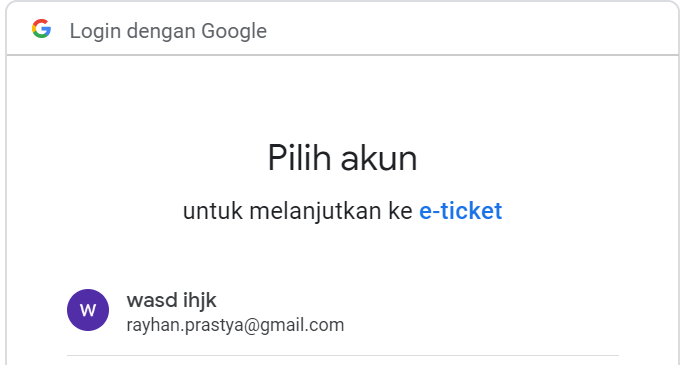
\includegraphics[scale=0.5]{gambar/gugel}
    \caption{\textit{Masuk Akun Google}}
    \label{gugel}
\end{figure}

\section{Pengujian}

\subsection{\textit{Black Box}}

\begin{table}[]
\captionsetup{singlelinecheck=off}
\caption{Blackbox}
\label{blackbox}
\begin{tabular}{|l|l|l|l|l|l|l|}
\hline
\multirow{2}{*}{Kelas}      & \multirow{2}{*}{\begin{tabular}[c]{@{}l@{}}Butir \\ Uji\end{tabular}}           & \multicolumn{2}{l|}{Identifikasi}           & \multirow{2}{*}{\begin{tabular}[c]{@{}l@{}}Tingkat \\ Pengujian\end{tabular}} & \multirow{2}{*}{\begin{tabular}[c]{@{}l@{}}Jenis \\ Pengajuan\end{tabular}} & \multirow{2}{*}{Jadwal}     \\ \cline{3-4}
                            &                                                                                 & \multicolumn{2}{l|}{PDHUPL}                 &                                                                               &                                                                             &                             \\ \hline
\multirow{2}{*}{Lingkungan} & \multirow{2}{*}{\begin{tabular}[c]{@{}l@{}}Halaman \\ Pendaftaran\end{tabular}} & \multicolumn{2}{l|}{\multirow{2}{*}{A\_01}} & \multirow{2}{*}{\begin{tabular}[c]{@{}l@{}}Pengujian \\ Sistem\end{tabular}}  & \multirow{2}{*}{\begin{tabular}[c]{@{}l@{}}Black \\ Box\end{tabular}}       & \multirow{2}{*}{19/07/2019} \\
                            &                                                                                 & \multicolumn{2}{l|}{}                       &                                                                               &                                                                             &                             \\ \hline
\end{tabular}
\end{table}

\par
Berikut pada tabel \ref{blackbox}, merupakan pengujian dengan melakukan metode \textit{blackbox}

\begin{table}[!htbp]
    \captionsetup{singlelinecheck=off}
       \caption{\textit{Masuk Akun Google}}
    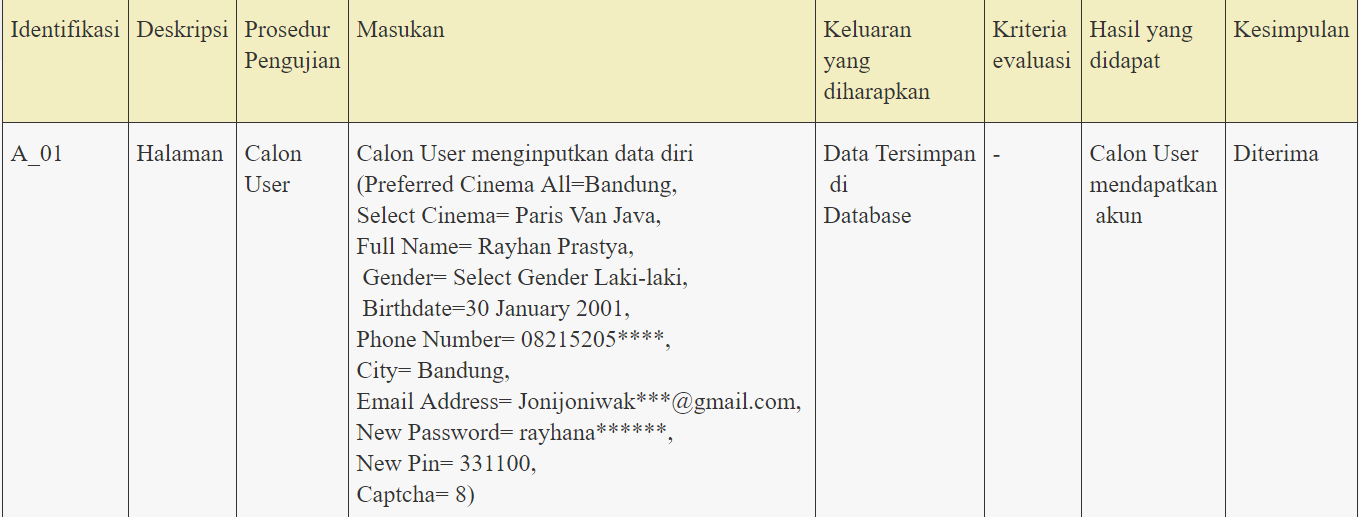
\includegraphics[scale=0.3]{gambar/black}
    \label{black}
\end{table}